\scanpage{26}
\[
u_+ \qquad \frac{1}{2}(u_++u_-)
\]

\[
\underset{m}{\underset{\rule{.35pt}{2pt}\rule{4.4em}{.35pt}\rule{.35pt}{2pt}}{(x+\tfrac{1}{2}y)}}u_+
+\underset{n}{\underset{\rule{.35pt}{2pt}\rule{2em}{.35pt}\rule{.35pt}{2pt}}{\tfrac{1}{2}y}}u_-
\]

\figure{
\begin{tikzpicture}[x=.6cm,y=.6cm,line cap=round,line join=round]
\draw[gray,line width=3pt] (.1,2.5) .. controls (-.5,4.3) and (.4,4.7) .. (1.6,4.1) .. controls (.7,4.6) and (.1,4.1) .. (.1,2.5) .. controls (.7,3.6) and (1.5,3.7) .. (2.1,3.2) -- (1.95,4.6) -- (.45,.2) -- (1.95,4.6) -- (1.5,1.1) .. controls (1.2,1.4) and (-.5,1.7) .. (1.95,4.6) -- (0,0);
\draw[gray,line width=3pt] (1.3,.3) .. controls (1.55,1.7) and (1.15,2.7) .. (1.85,2.65) .. controls (2.15,2.7) and (2.4,2.5) .. (2.5,2.1);
\end{tikzpicture}}

\diagram{\begin{tikzcd}[ampersand replacement=\&,column sep=small]
0 \arrow[r] \& \Pi \arrow[r] \& V \arrow[r,dash] \& E \arrow[r] \& 0
\end{tikzcd}}

\[
H^1(\deleted{\unsure{\langle}}\gamma,E)\xrightarrow{\sim} H^{\unsure{2}}(\gamma,\Pi)\simeq \Pi^{\gamma}/(1+\sigma)(\Pi)
\]

\[
z\longmapsto\exp 2i\pi z
\]

\figure{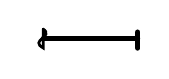
\begin{tikzpicture}[x=1cm,y=1cm,line cap=round]
\draw[line width=1.8pt] (0,0)--(1.2,0);
\draw[line width=1pt] (0,.12)--(0,-.12) .. controls (-.18,-.02) and (.14,.02) .. (0,.12);
\draw[line width=2pt] (1.2,-.12)--(1.2,.08);
\end{tikzpicture}}
% archive sheet number: 28
